\documentclass[11pt, journal]{IEEEtran}

\usepackage{lipsum}
\usepackage[T1]{fontenc}
\usepackage{fouriernc}
\usepackage{cases}
\usepackage{amsmath}
\usepackage{amssymb}
\usepackage[noadjust]{cite}
\usepackage{hyperref}
\usepackage{multirow}
\usepackage{graphicx}
\usepackage{adjustbox}
\usepackage{makecell}
\usepackage[table, dvipsnames]{xcolor}
\usepackage{tikz}
\usepackage{lipsum}
\usepackage{listings}
\usepackage{fontawesome5}
\usepackage{tcolorbox}
\usepackage[table, dvipsnames]{xcolor}
\usepackage[ruled]{algorithm2e}
\usepackage{array}
%\usepackage{caption}
\usepackage{bibtex}
\usepackage{cite}

%\addbibresource{bibliography.bib}

\hypersetup{
    colorlinks=true,
    linkcolor=blue,
    anchorcolor=blue,
    urlcolor=blue,
    citecolor=blue
}

\definecolor{codeCOMMENT}{HTML}{649541}
\definecolor{codeSTRING}{HTML}{37864A}
\definecolor{codeKEY}{HTML}{C678DD}
\definecolor{codeFUNC}{HTML}{61AFEF}
\definecolor{codeVALUES}{HTML}{C69438}

\newcommand{\eq}{\; = \;}
\newcommand{\nwl}{

\vspace{11pt}

}
\newcommand{\centered}[2]{\begin{tabular}{#1} #2 \end{tabular}}

\lstdefinestyle{standstyle}{
    commentstyle=\color{codeCOMMENT},
    keywordstyle=\bfseries\color{codeKEY},
    numberstyle=\scriptsize\ttfamily\color{codeVALUES},
    stringstyle=\color{codeSTRING},
    basicstyle=\ttfamily\linespread{1}\scriptsize\color{black!80},
    breakatwhitespace=false,
    breaklines=true,
    captionpos=b,
    keepspaces=true,
    numbers=left,
    numbersep=5pt,
    showspaces=false,
    showstringspaces=false,
    showtabs=false,
    tabsize=4,
    xleftmargin=15pt,
}

\lstset{style=standstyle}

%\newfloat{Code}{htbp}{loa}

\DeclareMathAlphabet{\mathcal}{OMS}{zplm}{m}{n}
\DeclareMathOperator*{\argmax}{arg\,max}
\DeclareMathOperator*{\argmin}{arg\,min}

\newcommand{\norm}[1]{\left\lVert#1\right\rVert}
\newcommand\commentalg[1]{\textcolor{ForestGreen}{{\footnotesize #1}}}
\SetCommentSty{commentalg}

\title{$k$-means is (\textit{really}) all you need}
\author{Leonardo Biason ($2045751$) \quad Alessandro Romania ($2046144$)}

\begin{document}

\maketitle

\begin{abstract}
    The $k$-means algorithm is a well known clustering algorithm, which is often used in unsupervised learning settings. However, the algorithm requires to perform multiple times the same operation on the data, and it can greatly benefit from a parallel implementation, so that to maximize the throughput and reduce computation times. With this project, we propose some possible implementations, based on some libraries that are considered to be the \text{de-facto} standard when it comes to writing multithreaded or parallel code, and we will discuss also the results of such implementations
\end{abstract}

\begin{keywords}
    Sapienza, ACSAI, Multicore Programming
\end{keywords}
\nwl
%\begin{tcolorbox}[colback = Purple!20, colframe = Purple!40]
%    \begin{center}
%        \faIcon{github} Check our repository \href{https://www.github.com/ElBi21/PSEM-kmeans}{on GitHub}
%        \verb|ElBi21/PSEM-kmeans|
%    \end{center}
%\end{tcolorbox}

\section{Introduction}

When talking about clustering and unsupervised learning, it's quite common to hear about the $k$-means algorithm, and for good reasons: it allows to efficiently cluster a dataset of $d$ dimensions, and it employs the notion of convergence in order to do so. This, computationally speaking, means to repeat some operations over and over again until some stopping conditions are met.
\nwl
The algorithm is not perfect though, and presents some issues:
\begin{itemize}
    \item [1)] the algorithm is fast in clustering, but we cannot be certain that it clusters \textit{well};
    \item [2)] the algorithm doesn't work with non-linear clusters;
    \item [3)] the initialization can make a great impact in the final result.
\end{itemize}
\nwl
Many people prefer to use other clustering methods, such as the fitting of Gaussian Mixture Models. Albeit not being perfect, $k$-means still works well in simple, linear clusters. For the sake of this project, we are going to consider a vanilla $k$-means algorithm with Lloyd's initialization (the first $k$ centroids will be selected randomly).

\subsection{Algorithm structure}

The $k$-means algorithm can be described with the following pseudocode, where $X$ is the set of data points, $C = \{\mu_1, \; \mu_2, \; ..., \; \mu_k \}$ is the set of centroids and $Y$ is the set of assignments:

\begin{algorithm}
    \label{algkmeans}
    \LinesNumbered
    \tcp{Initialize the centroids}
    \For{$k$ in $[1, \; |C|]$}{
        $\mu_k \gets \text{a random location in the input space}$
    }
    \BlankLine
    \While{$\text{convergence hasn't been reached}$}{
        \tcp{Assign each point to a cluster}
        \For{$i$ in $[1, \; |X|]$}{
            $y_i \gets \argmin_k \left(\norm{\mu_k - x_i}\right)$ 
        }
        \BlankLine
        \tcp{Compute the new position of each centroid}
        \For{$k$ in $[1, \; |C|]$}{
            $\mu_k \gets \textsc{Mean}(\{ \; x_n : z_n = k \; \})$
        }
    }
    \tcp{Return the centroids}
    \Return $Y$

    \caption{$k$-means (Lloyd's initialization)}
\end{algorithm}

The algorithm consists of 4 main blocks:
\begin{itemize}
    \item the \textbf{initialization block}, where all the centroids will receive a starting, random position (as per Lloyd's method);
    \item the \textbf{assignment block}, where the Euclidean distance between a point and all centroids is computed, for all centroids. The point will be assigned to a cluster depending on the following operation:
    \[ \argmin_k \left(\norm{\mu_k - x_i}\right) \]

    \item the \textbf{update block}, where the position of the centroids is updated, and the new position of a centroid $\mu_k$ is equal to the mean of all the data points positions belonging to cluster $k$
\end{itemize}

\subsection{Sequential Code Bottlenecks}

For implementing the $k$-means algorithm, we will base all the codebase upon the project made from professors Diego García-Álvarez and Arturo Gonzalez-Escribano from the University of Valladolid \cite{kmeans-univallo}. The code shown in this subsection is taken from their project, although slightly adapted for giving enough context in the code snippets.
\nwl
We described before the overall structure of the $k$-means algorithm: we will now proceed to examine its two main bottlenecks. As we can see from Algorithm \ref{algkmeans}, we have two main blocks that may cause performance issues: the \textbf{assignment block} and the \textbf{update block}.
\nwl
The first \textbf{for} block in the \textbf{initialization step} does not represent a major bottleneck, since it just needs to assign a random location to each of the $K$ centroids. It can be parallelized, but it won't help as much as parallelizing the two steps mentioned before.
\nwl
The second \textbf{for} block represents the \textbf{assignment step}, which is, unlike the initialization step, computationally expensive: for each point, the algorithm will have to compute the euclidean distance (here onwards denotes as $\ell_2$) between said point and all centroids $\mu_k \in C$, and select the lowest distance. This will determine the cluster of the point. In a C program, this may be accomplished with the following piece of code:
\nwl
\begin{lstlisting}[language = C]
int cluster;
// For each point...
for(i = 0; i < points_number; i++) {
    class = 1;
    minDist = FLT_MAX;
    // For each cluster...
    for(j = 0; j < K; j++) {
        // Compute the distance
        dist = l2_norm(&data[i*samples], &centroids[j*samples], samples);

        // If the distance is the lowest so far, replace it
        if(dist < minDist) {
            minDist = dist;
            class = j+1;
        }
    }
    
    // If the class is different from before, add a change to the counter
    if(classMap[i] != class) {
        changes++;
    }

    classMap[i]=class;
}\end{lstlisting}

Notice the presence of the two nested \textbf{for} loops: sequentially, they would take a time of $O(|X| \cdot |C|)$, which may be optimized just by taking a simple single instruction multiple data approach (indeed, with $m > 1$ different processes or threads, it would take a time of $O\left(\frac{|X| \cdot |C|}{m}\right)$ each, which is already better than the first option).
\nwl
The third \textbf{for} loop represents the update step, which also is computationally expensive: we would need to perform the mean of the coordinates of all the points belonging to a cluster $\mu_k$. This implies that all the coordinates of the points must be first summed, and then averaged on the number of points being classified to $\mu_k$. An implementation in the C language would look like the following:
\nwl
\begin{lstlisting}[language = C]
// For each point...
for (i = 0; i < lines; i++) {
    point_class = classMap[i];
    // Add 1 to the points classified for class k
    pointsPerClass[point_class - 1] += 1;

    // For each dimension...
    for(j = 0; j < samples; j++) {
        // ...add it to a table for summing and averaging
        auxCentroids[(point_class - 1) * samples + j] += data[i * samples + j];
    }
}

for (i = 0; i < K; i++) {
    for (j = 0; j < samples; j++) {
        // Average all dimensions
        auxCentroids[i * samples + j] /= pointsPerClass[i];
    }
}

maxDist = FLT_MIN;
for (i = 0; i < K; i++) {
    // Compute the moving distance, as a convergence check
    distCentroids[i] = euclideanDistance(&centroids[i * samples], &auxCentroids[i * samples], samples);
    if (distCentroids[i] > maxDist) {
        maxDist = distCentroids[i];
    }
}\end{lstlisting}

\subsection{Performance evaluation}

\begin{table}
    \label{seq_times}
    \centering
    \caption{Runtime of the sequential version $\left(\mu \pm \sigma^2\right)$}
    \renewcommand{\arraystretch}{1.3}
    \begin{tabular}{|c|c|c|}
        \hline
        \multicolumn{3}{|c|}{\textbf{Input tests}} \\
        \hline\hline
        20D & 100D & 100D$_2$ \\
        \hline
        $0.35398 \pm 0.00019$ & $1.06496 \pm 0.00061$ & $111.27844 \pm 0.06059$ \\
        \hline
    \end{tabular}
\end{table}

All the following codes have been tested on Sapienza's internal cluster, where for each node an \textbf{AMD EPYC 7301 CPU} is mounted (which has up to \textbf{64 logical cores}). In some cases, nodes with NVIDIA GPUs can be requested, and the used GPU is the \textbf{RTX Quadro 6000}, which has a compute capability of 7.5; for this reason, the CUDA program is compiled with that architecture in mind, so newer features of other CUDA architectures haven't been taken into account.
\nwl
For each program, we tested the applications for 30 times on 3 different tests: 20D, 100D and 100D$_2$. The programs were launched with the following test:

\begin{center}
    \verb|<test_file> 30 500 0.1 0.1 <out>|
\end{center}

All the measured values can be found at the end of this report in multiple tables, which will be referenced throughout the paper. Specifically, the timings are reported in the form $\mu \pm \sigma^2$, where $\mu$ stands for the mean and $\sigma^2$ for the standard deviation. In the timing plots, we haven't reported the standard deviations, due to the fact that they were not properly readable; such values can be however found in the tables.
\nwl
The \textbf{speedup} $S_{d, t}$ (where $T$ stands for the timing, $d$ for the test and $t$ for the number of threads/processes used) and the \textbf{efficiency} $E_{d, t}$ have also been reported. Such values have been computed with the following formulas:
\[ S_{d, t} = \frac{T_{\text{serial}, \; d}}{T_{\text{parallel}, \; d, t}} \quad \quad E_{d, t} = \frac{S_{d, t}}{t} \]

Lastly, we haven't considered the Ahmdahl and Gustafson laws in the evaluation, since the vast majority of our computations have been parallelized. While there are a few operations that have been done sequentially, they are negligible with respect to the programs' workloads.

\section{Parallelizing with MPI}

The \textbf{Message Passing Interface} (\textbf{MPI}) is a standardized, portable framework that enables parallel computation across distributed memory systems. These systems, typically clusters of interconnected computers, do not share a common memory. Each process operates on its local memory and must explicitly communicate with others by sending and receiving messages. MPI achieves parallelism through process-based communication, distributing both data and tasks among multiple processes.
\nwl
Achieving efficient parallel performance in MPI programs requires attention to two critical factors:
Balancing the workload across processes
Minimizing the frequency of message passing
Both factors are crucial for scalable and high-performance parallel applications. Here's how these optimizations are implemented in this $k$-means clustering algorithm:

\subsection{MPI Implementation Approach}
The $k$-means clustering program follows a \textbf{Globally Parallel, Locally Sequential} (\textbf{GPLS}) model. This means that the critical initialization and termination tasks are handled by rank 0, while the looping part of the algorithm is entirely parallelized.
\nwl
\subsubsection{Initialization phase}
In the initialization phase is where workload balancing decisions are made.
Rank 0 reads the input data from a file (as only rank 0 has access to the file).
The input data (points) is broadcast to all processes using \verb|MPI_Scatterv|. The points remain fixed throughout the execution, enabling a single communication step to distribute data efficiently. The Centroids are randomly generated by rank 0. These centroids are then broadcasted to all processes.
\nwl
\subsubsection{Loop phase}
The loop phase involves two key operations that are parallelized over different data structures:
\begin{itemize}
    \item \textbf{point assignment}: each process works on its local points with its local classMap. This assignment step is fully parallel, as each process handles its portion of the points independently. Assignment changes are accumulated locally and reduced globally using \verb|MPI_Iallreduce| for checking at the and the termination conditions;
    \item \textbf{centroid update}: once all points are assigned, each process calculates local partial sums for centroids and the number of points in each cluster. These partial results are aggregated across all processes using \verb|MPI_Allreduce|, ensuring globally consistent centroid values with fast communication. Each process then updates its locally assigned centroids based on the reduced global values, distributing the workload evenly among processes. The maximum distance between old and updated centroids is calculated locally and reduced globally using \verb|MPI_Allreduce| to check for termination conditions. After these checks, an \verb|MPI_Allgatherv| operation gathers all local centroids, preparing them for the next iteration.
\end{itemize}

\subsubsection{Termination phase}

In the termination phase, local point assignments (the output of the $k$-means algorithm) are gathered by the rank 0 process using \verb|MPI_Gather|. Finally, all processes free their allocated memory, and the algorithm terminates.

\begin{figure}
    \label{mpi_speedup_eff}
    \centering
    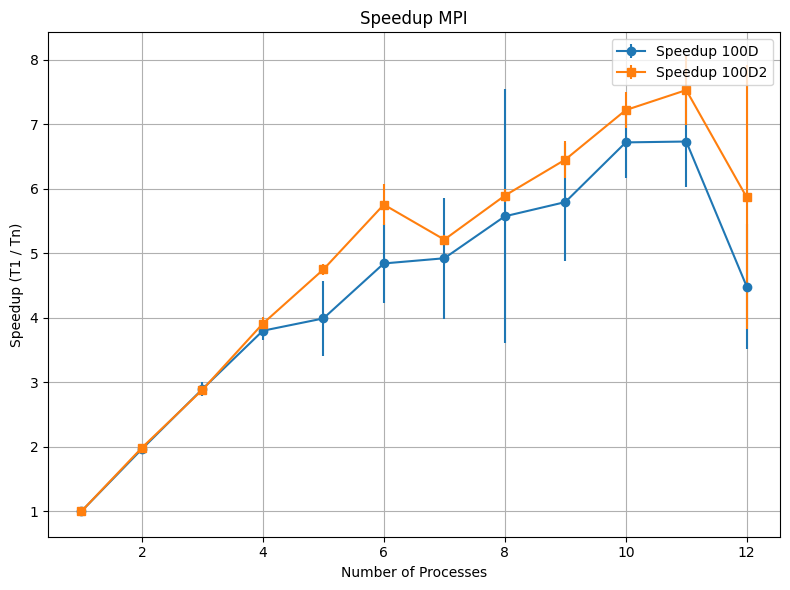
\includegraphics[width=\linewidth]{imgs/mpi_speedup.png}
    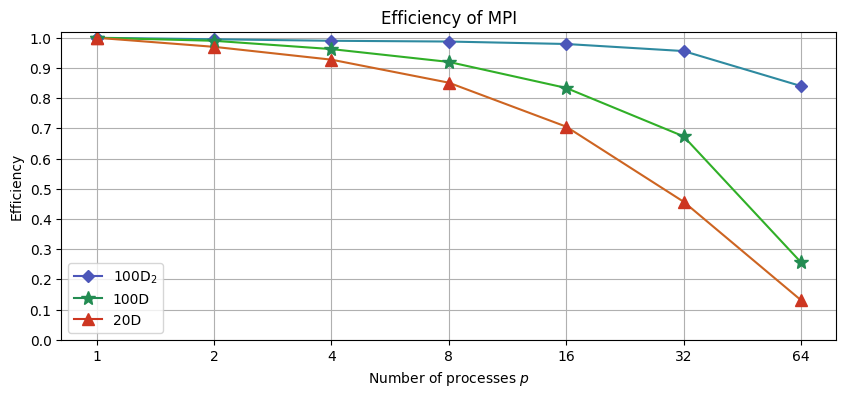
\includegraphics[width=\linewidth]{imgs/mpi_efficiency.png}
    \caption{Speedup (top image) and efficiency (bottom image) of the MPI application with three different tests}
\end{figure}

\subsection{MPI Performance Analysis}

We tested with 1, 2, 4, 8, 16, 32 and 64 MPI processes. The MPI program achieves nearly linear speedup across all input sizes up to 16 processes. For the largest input size (100D$_2$), the speedup continues to increase steadily up to 32 processes and maintains a near-linear trend even up to 64 processes. This indicates that for large-scale problems, the computation-to-communication ratio remains favorable, allowing the system to scale efficiently. However, for the smaller input sizes (100D and 20D), the speedup begins to decrease after 32 processes, as can be seen in figure \ref{mpi_speedup_eff}. This drop in performances is primarily due to the increasing overhead of inter-process communication and memory exchange. As the number of processes grows, the amount of data each process handles becomes smaller, and the cost of communication dominates, making parallelism not efficient as we can see in table \ref{mpi_timings_table} for MPI.
\nwl
Considering weak and strong scaling, the program exhibits both characteristics to some extent. It demonstrates strong scaling effectively up to 16 processes, particularly for larger problem sizes, where the speedup remains close to linear as more processes are added (100D$_2$). However for smaller input sizes the overhead from inter-process communication begins to outweigh the benefits of parallelism, leading to diminishing returns. In terms of weak scaling, the program performs well for larger input sizes, as it maintains relatively consistent performance when both the problem size and the number of processes increase proportionally. 
\nwl
The MPI implementation is well-suited for handling large-scale computations where the computation-to-communication ratio remains high. Overall, the MPI program scales efficiently, but its scalability is ultimately bounded by communication overhead at higher process counts for smaller datasets.


\section{Parallelizing with PThread}

\textbf{POSIX Threads} (\textbf{PThreads}) is an API defined by the POSIX standard, providing a powerful and flexible framework for parallel programming on shared memory systems. PThreads give developers low-level control over threads creation, synchronization, and data sharing. Each thread represents an independent flow of execution, and all threads within a process share the same memory space, making inter-thread communication efficient but also more complex to manage. PThreads require explicit management of thread lifecycle, workload division, synchronization primitives (like mutexes, condition variables, and barriers), and memory consistency. While this manual control allows for highly customized parallel solutions, it also increases the potential for bugs such as race conditions or deadlocks if not handled carefully.

\subsection{PThread Implementation Approach}

For implementing the PThread version, we aimed at creating a unique function, which would contain the main loop of the algorithm. In order to do that, we made use of the PThread barriers, which can be optionally activated through a flag in the program. In order to pass the parameters to the threads, two structs have been created, one for global parameters (whose pointer is shared with all threads) and one for local parameters. In order to split the workload, each thread first gets assigned a quantity of data points and centroids; this quantity is computed as follows:
\[ \texttt{local\_n} = \left\lfloor \frac{n}{t} \right\rfloor \quad \quad \texttt{local\_k} = \left\lfloor \frac{k}{t} \right\rfloor \]

After that, if there are any remaining data points/centroids (so if there exists a remainder of the previous division which is not 0), they get assigned to multiple threads in a round-robin fashion. This computation is done by the program before launching the threads.
\nwl
In the kernel, if a thread has a \verb|local_n| $> 0$, then it can participate to the computation of the first step of the algorithm, so assigning the points to a cluster. If the thread doesn't participate, it skips the step and waits for all other threads. After the first step, a barrier will make sure that all threads have completed the tasks assigned so far; then, through a lock, the points per class and the coordinates of the auxiliary centroids that were computed locally get summed.
\nwl
Similarly for the first step, only all threads with \verb|local_k| $> 0$ can participate to the computation of the second step. In the second step each thread computes the new centroids, first by averaging the coordinates of the assigned auxiliary centroids, and then by computing the new distances (for the convergence check). After that, a barrier will wait for all threads to finish, and then through a second lock the convergence parameters get updated. 

\subsection{PThread Performance analysis}

The PThread program was tested with 1, 2, 4, 8, 16, 32 and 64 threads. The runtimes can be observed both in figure \ref{mpi_pt_runtimes} and in table \ref{pt_timings_table}. The speedup and the efficiency of the PThread implementation reach high values, especially with high quantities of data: indeed, the speedup is nearly linear even with 32 threads with the test 100D$_2$ (by table \ref{mpi_pt_speedup_table}, we have $31.28\times$) The plots in figure \ref{pt_speedup_eff} help highlighting the strong scaling of the application. Similarly to the MPI application, after 32 threads with the smaller tests (20D and 100D) the application performances (both the efficiency and speedup) start decreasing. The main reason of this is due to the overhead of instantiating multiple threads which do too few operations, and that need to synchronize in multiple parts of the application. We can also notice some properties of weak scalability: by the augmentation of the number of threads and of the sizes of the problem, the speedup and efficiency increase as well, and this can be ultimately noticed by the values in table \ref{mpi_pt_speedup_table}.

\begin{figure}
    \label{pt_speedup_eff}
    \centering
    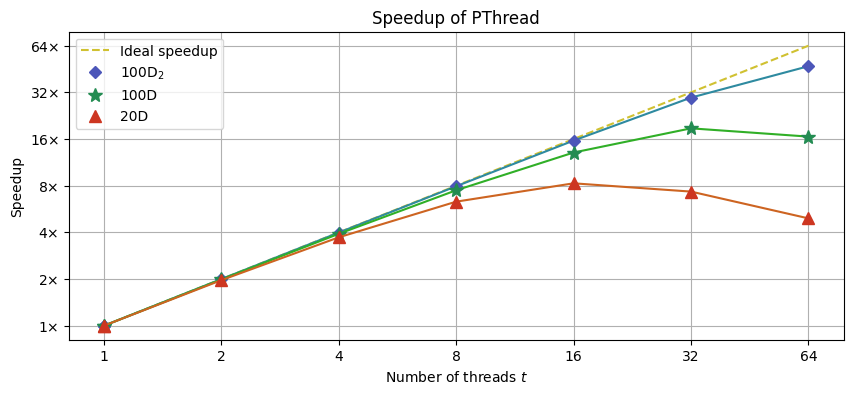
\includegraphics[width=\linewidth]{imgs/pt_speedup.png}
    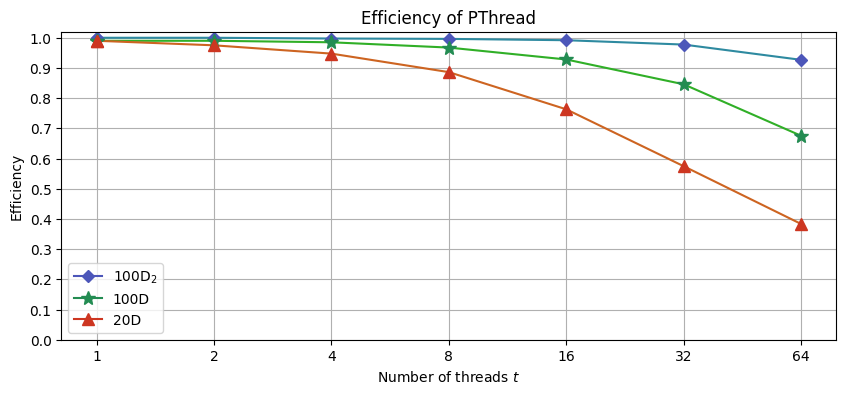
\includegraphics[width=\linewidth]{imgs/pt_efficiency.png}
    \caption{Speedup (top image) and efficiency (bottom image) of the PThread application with three different tests}
\end{figure}

\begin{figure*}
    \label{mpi_pt_runtimes}
    \centering
    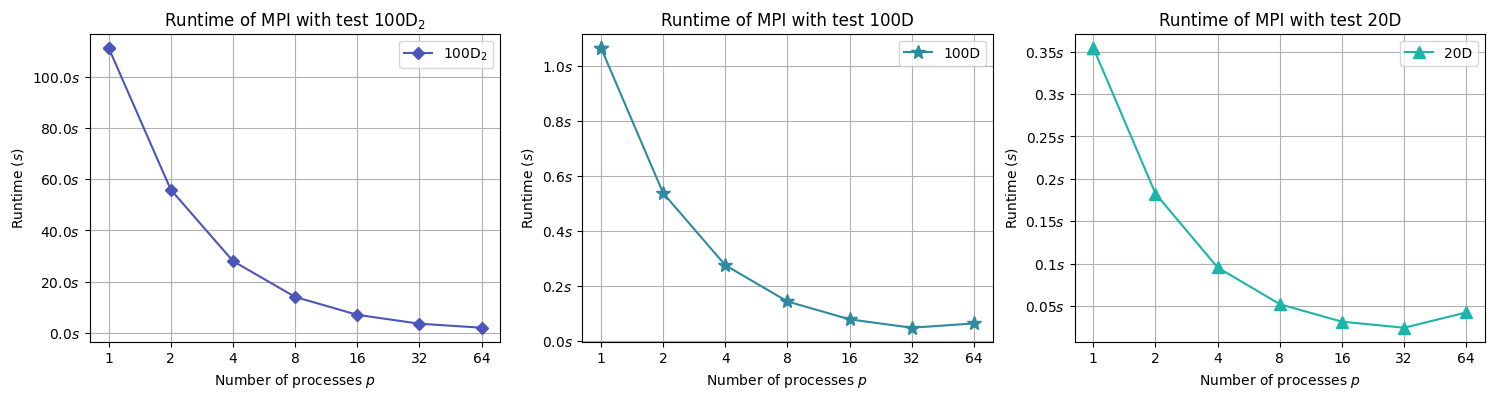
\includegraphics[width=\linewidth]{imgs/mpi_runtime.png}
    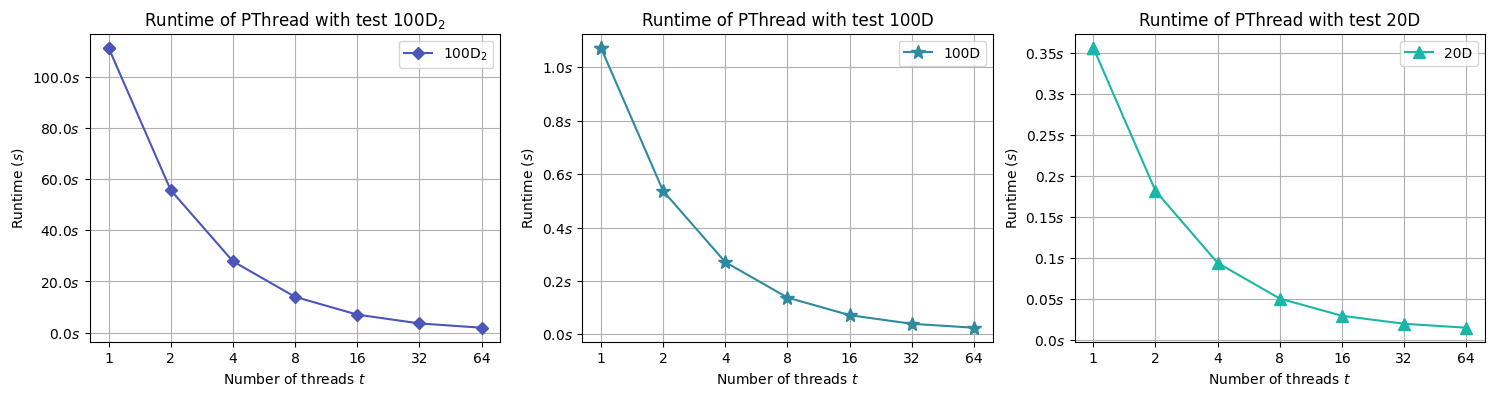
\includegraphics[width=\linewidth]{imgs/pt_runtime.png}
    \caption{Runtimes of the MPI and PThread applications with three different tests}
\end{figure*}

\section{Parallelizing with CUDA}

In recent years, we have seen how GPUs play crucial roles when it comes to parallelizing a program with multiple threads. Indeed, the model proposed by NVIDIA for its CUDA platforms (namely, the Single-Thread Multiple-Data model) turned out to be very efficient, by allowing notable speed-ups and augmentation of the throughput. Clearly, this can be applied also to the $k$-means algorithm, and we'll now proceed to illustrate our proposed model.

\subsection{Designing the parallel structure}

As we have shown in Algorithm \ref{algkmeans}, the $k$-means algorithm can be logically split into two steps: the assignment step and the update step. However, while logically this division may sound reasonable, it is not appropriate for the STMD model that NVIDIA has at the core of its devices, and this is because of the data needed by the two steps:
\begin{itemize}
    \item the \textbf{assignment step} needs to work only with the data points, but can be parallelized by splitting the data into multiple parts;
    \item the \textbf{update step} instead needs to work with both all the data and all the centroids, so parallelizing the step as a whole becomes quite hard.
\end{itemize} 

A simpler approach would be to split the update step in two parts, one which distributes the points over the threads, and another that distributes the centroids. This would create in total three parallelization steps. In our implementation, such steps are developed in the following three kernels: \verb|assignment_step|, \verb|update_step_points| and \verb|update_step_centroids|.

\subsection{Program parameters, custom \texttt{atomicMax} and memory management}

We decided to organize the threads in two dimensional blocks of $32 \times 32$ threads, and the blocks are instead organized in a one dimensional grid. The size of the grid is dynamically determined depending on the called kernel: usually, we have that $|X| \gg k$, so it's pointless for CUDA to reserve a grid of threads for the centroids that has the same size of the grid of the points. The grids' dimensions are computed following these formulas:

\[ \texttt{points\_grid\_size} \; = \; \frac{\left| X \right|}{32 \times 32} + 1 \]
\[ \texttt{centroids\_grid\_size} \; = \; \frac{k}{32 \times 32} + 1 \]

The program makes also use of a custom function, called \verb|custom_atomic_max()|. This function has been implemented because it allows us to perform an \verb|atomicMax()|-like function for \verb|float| numbers, which would not be normally possible with the built-it CUDA function. We here show the function as a whole:
\nwl
\begin{lstlisting}[language = C]
__device__ float custom_atomic_max(float* value_address, float val) {
    int* address_as_int = (int*) value_address;
    int old = *address_as_int, assumed;
    do {
        assumed = old;
        old = atomicCAS(address_as_int, assumed, __float_as_int(fmaxf(val, __int_as_float(assumed))));
    } while (assumed != old);
    return __int_as_float(old);
}\end{lstlisting}
\nwl
The idea of the function is that CUDA tries continuously to perform an \verb|atomicCAS()| operation, which in turns performs atomically the following check:
\begin{center}
    \scriptsize
    \verb|old_value == to_compare ? new_value : old_value|
\end{center}

The function will exit only when the value in the specified address is equal to the one that the program expects to be there, before performing the atomic transaction. This is important, so that to avoid that the function overwrites any unintentional value.
\nwl
Especially with CUDA, a great part of the possible sppedup that an application can achieve is given by the memory accesses. One of the many possibilities that CUDA offers, that is not instead possible with CPUs (be it with multi-processing or multi-threading programming), is to \textbf{freely manage} the \textbf{L2 cache} of the GPU (also known as the shared memory). In our implementation, we made sure to use the shared memory as much as possible, and to transfer the data to the global memory only when needed. Moreover, we made sure to use most efficiently the \textbf{memory coalescing} that CUDA does whenever retrieving data from the global memory: this has been done by "transposing" the \verb|data| array. Normally, the \verb|data| array would be organized as follows:

\begin{center}
    \resizebox{\linewidth}{!}{
        \renewcommand{\arraystretch}{1.3}
        \begin{tabular}{c|c|c|c|c|c|c|c}
            \cline{2-4}\cline{6-7}
            $\Longrightarrow$ & $p_{1, \; 1}$ & $p_{1, \; 2}$ & $p_{1, \; 3}$ & $...$ & $p_{1, \; d-1}$ & $p_{1, \; d}$ & $\hookleftarrow_1$ \\
            \cline{2-4}\cline{6-7}
            $\hookrightarrow_1$ & $p_{2, \; 1}$ & $p_{2, \; 2}$ & $p_{2, \; 3}$ & $...$ & $p_{2, \; d-1}$ & $p_{2, \; d}$ & $\hookleftarrow_2$ \\
            \cline{2-4}\cline{6-7}
            \multicolumn{1}{c}{} & \multicolumn{3}{c}{$\vdots$} & \multicolumn{1}{c}{$\ddots$} & \multicolumn{2}{c}{$\vdots$} & \\
            \cline{2-4}\cline{6-7}
            $\hookrightarrow_{n-1}$ & $p_{n, \; 1}$ & $p_{n, \; 2}$ & $p_{n, \; 3}$ & $...$ & $p_{n, \; d-1}$ & $p_{n, \; d}$ & \\
            \cline{2-4}\cline{6-7}
        \end{tabular}
    }
\end{center}

\nwl
where the notation $p_{i, \; j}$ stands for the $j^{\text{th}}$ coordinate of the $i^{\text{th}}$ point; in other words, the array was originally stored point-wise (so first all the $d$ coordinates of the first point, then the $d$ coordinates of the second point, and so on...). After transposing the array, it became as follows:

\begin{center}
    \resizebox{\linewidth}{!}{
        \renewcommand{\arraystretch}{1.3}
        \begin{tabular}{c|c|c|c|c|c|c|c}
            \cline{2-4}\cline{6-7}
            $\Longrightarrow$ & $p_{1, \; 1}$ & $p_{2, \; 1}$ & $p_{3, \; 1}$ & $...$ & $p_{n-1, \; 1}$ & $p_{n, \; 1}$ & $\hookleftarrow_1$ \\
            \cline{2-4}\cline{6-7}
            $\hookrightarrow_1$ & $p_{1, \; 2}$ & $p_{2, \; 2}$ & $p_{3, \; 2}$ & $...$ & $p_{n-1, \; 2}$ & $p_{n, \; 2}$ & $\hookleftarrow_2$ \\
            \cline{2-4}\cline{6-7}
            \multicolumn{1}{c}{} & \multicolumn{3}{c}{$\vdots$} & \multicolumn{1}{c}{$\ddots$} & \multicolumn{2}{c}{$\vdots$} & \\
            \cline{2-4}\cline{6-7}
            $\hookrightarrow_{d-1}$ & $p_{1, \; d}$ & $p_{2, \; d}$ & $p_{3, \; d}$ & $...$ & $p_{n-1, \; d}$ & $p_{n, \; d}$ & \\
            \cline{2-4}\cline{6-7}
        \end{tabular}
    }
\end{center}

\nwl
thus having a data array where the \textbf{coordinates} are \textbf{stored dimension-wise} (so first the first dimension of all the points, then the second dimension, and so on...). This is preferrable since, when computing the new centroids, all threads will work "simultaneously" on the same dimension of the data, so when recovering the data coordinates from the global memory the GPU will load a burst of coordinates who belong to the same dimension together. This, as we'll show later on, \textbf{improves greatly} the speedups and timings of the application. While this may have been done also on the centroids, it is not strictly necessary, since the centroids will be already stored in the shared memory when needed.

\subsection{Analysis of the kernels}

\begin{figure*}
    \label{cuda_runtimes_speedups}
    \centering
    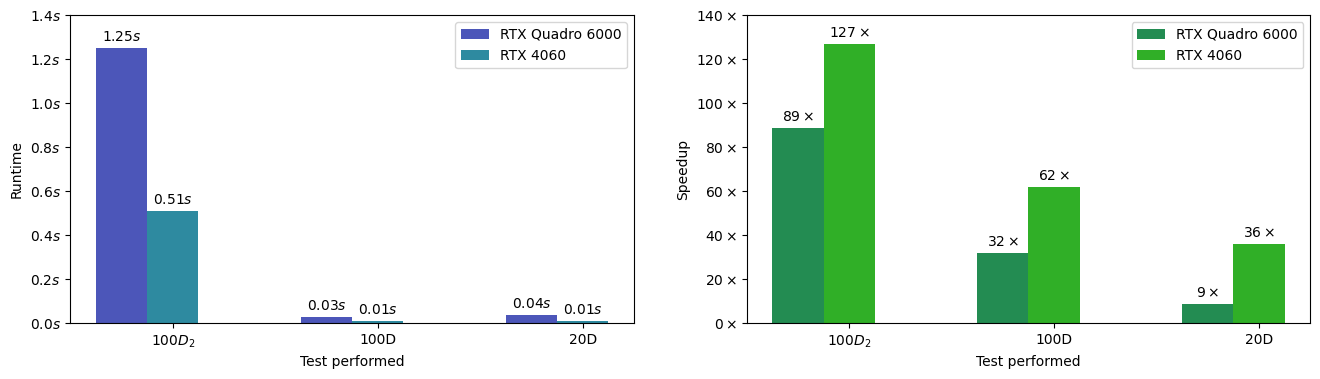
\includegraphics[width=\linewidth]{imgs/cuda_timings_speedups.png}
    \caption{Runtimes and speedups of the CUDA application on different GPUs}
\end{figure*}

As we mentioned previously, we are making use of three kernels: \verb|assignment_step| and \verb|update_step_points| and \verb|update_step_centroids|. In all kernels, all operations that act on the global memory are \textbf{performed atomically}, which avoid potential race conditions. We here show how all three kernels work.
\nwl
The first kernel is called on all the data, and each point is assigned to a thread. First, a preliminary check is performed, to make sure that each thread is assigned to a valid point. While the \verb|if| statement may seem like a possible cause of warp divergence, it doesn't actually impact that much. Indeed, we would only discard part of the final block of kernels, while all the previous blocks are fully used. Then, each thread will compute the $\ell_2$ norm between its assigned point and all centroids, and will store the class to which each point will be assigned into the \verb|class_int| variable, depending on which $\ell_2$ norm is the smallest. If a change from the previous class assignment is detected, the number of changes will increase.
\nwl
The second kernel will have a point assigned to each thread, and each thread will increment, in the \verb|points_per_class| array, the value in the position corresponding to the class assigned to the point. After that, the coordinates of the point are added to the \verb|aux_centroid| array, so that to create, on the new step, the new centroid from the average of the coordinates. Here, both the \verb|points_per_class| and \verb|aux_centroids| arrays are stored in shared memory, and only after a thread computes its contribution to the final array the result in shared memory gets copied over to the global memory (also here it is done through atomic operations, so that to avoid concurrency problems).
\nwl
The third kernel, \verb|update_step_centroids|, firstly ensure that all threads are mapped to a valid centroid; then all threads will compute, for each dimension of the centroids, the average coordinates of the new centroid. Once done, each thread will then perform the $\ell_2$ norm between the previous centroid and the new one, so that to compute the \verb|max_distance| variable, needed for convergence. Once again, the variable is first stored in shared memory, and it's then stored in global memory via the use of the \verb|custom_atomicMax()| function, which we illustrated previously.
\nwl
After executing the third kernel, the program continues repeating in loop the three kernels until one of the convergence conditions is met.

\subsection{CUDA Performance analysis}

The CUDA version performed as can be seen from table \ref{cuda_times}. As we mentioned in the previous section, the correct handling of the memory and exploitation of the memory bursts allows to reach high speedups of the application, as can be seen for the rows with the \textasteriskcentered$^{23}$ apex. In the table we also reported the timings and speedup of a version of the application that wasn't correctly exploiting memory coalescence: indeed, for that version the speedup is not as impactful as the speedups of the other versions. For the sake of comparison, we also sampled the performance of the application in other systems with other NVIDIA GPUs, such as an RTX 4060 (marked by \textasteriskcentered$^4$) and an RTX 5080 (marked by \textasteriskcentered$^5$); in such cases, the speedup is relative to the sequential timings obtained in the other systems.

% eventuale analisi del roofline model

\begin{table}
    \label{cuda_times}
    \centering
    \caption{Performances of the CUDA version $\left(\mu \pm \sigma^2\right)$}
    \renewcommand{\arraystretch}{1.3}
    \resizebox{\linewidth}{!}{
        \begin{tabular}{|c|c|c|c|}
            \hline
            \multirow{2}{*}{\textbf{Metric}} & \multicolumn{3}{c|}{\textbf{Input tests}} \\
            \cline{2-4}\cline{2-4}
             & 20D & 100D & 100D$_2$ \\
            \hline\hline
            \textbf{Runtime}$^{13}$ & $0.05633 \pm 0.02272$ & $0.12794 \pm 0.03329$ & $8.46844 \pm 1.29596$ \\
            \hline
            \textbf{Speedup}$^{13}$ & $6.28 \times$ & $8.32 \times$ & $13.14 \times$ \\
            \hline\hline \rowcolor{lightgray!40}
            \textbf{Runtime}$^{23}$ & $0.038851 \pm 0.00758$ & $0.03343 \pm 0.00402$ & $1.25401 \pm 0.00367$ \\
            \hline \rowcolor{lightgray!40}
            \textbf{Speedup}$^{23}$ & $9.11 \times$ & $31.86 \times$ & $88.74 \times$ \\
            \hline\hline
            \textbf{Runtime}$^{24}$ & $0.00545 \pm 0.00006$ & $0.00993 \pm 0.00004$ & $0.50741 \pm 0.00337$ \\
            \hline
            \textbf{Speedup}$^{24}$ & $35.92 \times$ & $61.9 \times$ & $126.83 \times$ \\
            \hline
        \end{tabular}
    }
    
    \nwl
    \textasteriskcentered$^1$: \textbf{without} a correct handling of memory coalescing\\
    \textasteriskcentered$^2$: \textbf{with} a correct handling of memory coalescing\\
    \textasteriskcentered$^3$: executed on an \textbf{RTX Quadro 6000}\\
    \textasteriskcentered$^4$: executed on a \textbf{GeForce RTX 4060}\\
    \textasteriskcentered$^5$: executed on a \textbf{GeForce RTX 5080}
\end{table}

\begin{figure*}
    \label{stats_mpi_omp}
    \centering
    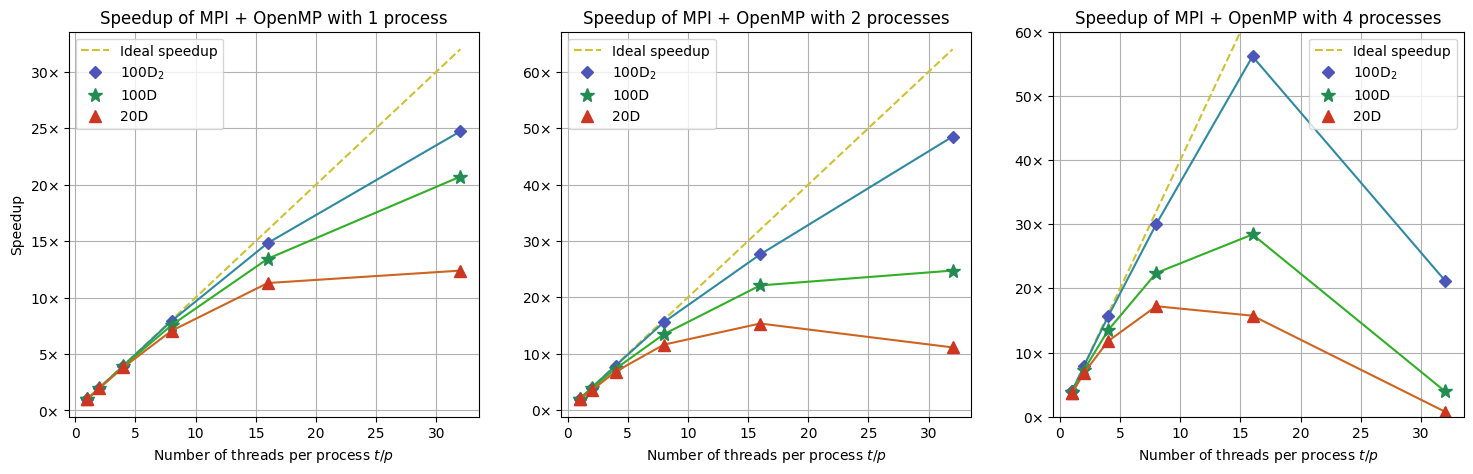
\includegraphics[width=\linewidth]{imgs/mpi_omp_speedup.png}
    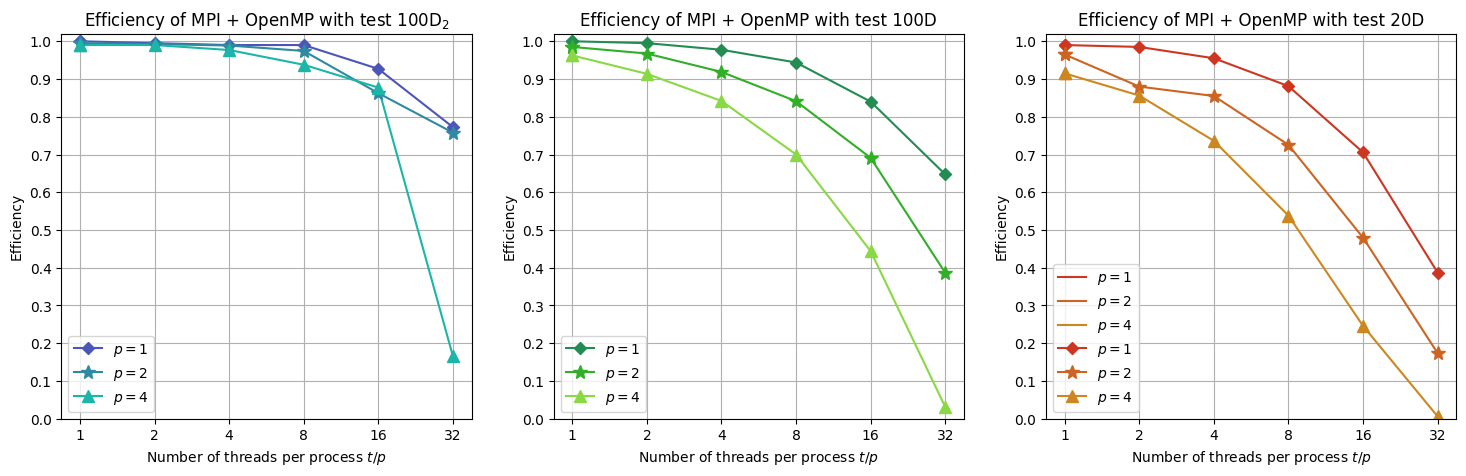
\includegraphics[width=\linewidth]{imgs/mpi_omp_efficiency.png}

    \caption{Comparison of the speedup of the MPI + OpenMP program (on top) and the efficiency (on bottom), on three different input tests. Each plot compares the program on a set amount of processes}
\end{figure*}

\section{Interlacing Multi-processing with Multi-threading with MPI + OpenMP}

So far, we implemented various solutions for our programs, which employed either multi-processing or multi-threading parallelism techniques, without using both approaches at the same time. However, these techniques are not mutually exclusive, and can be mixed together in order to achieve better performances. In fact, in high performance computing tasks, multi-process techniques are used within clusters to connect nodes and coordinate them, while multi-threading are used for performing computations, given the directives of the master process(es).
\nwl
In this section we will show how multi-threading approaches can be combined with the famous multi-processing library MPI, and this will be done thanks to the OpenMP library.
\nwl
The \textbf{Open Multi-Processing} (\textbf{OpenMP}) API is a standardized and portable framework designed to simplify parallel programming on shared memory systems, such as multi-core processors within a single machine. It enables efficient execution by allowing multiple threads to access a shared memory space. Threads can operate on either shared data or private copies, depending on the task. OpenMP achieves parallelism through simple compiler directives, allowing developers to parallelize sections of code without the complexity of manually managing threads, synchronization, or workload distribution.
\nwl
We implemented a version of the $k$-means algorithm that leverages both MPI and OpenMP to maximize performance. This hybrid approach is commonly used in cluster environments consisting of multiple nodes without shared memory. Within each node, OpenMP takes advantage of the shared-memory multiprocessor architecture, while MPI handles communication and data distribution across nodes.

\subsection{Implementation approach}

The $k$-means clustering program follows a Globally Parallel, Locally Sequential (GPLS) model. In this approach, the critical initialization and termination tasks are handled by rank 0, while the core looping part of the algorithm is fully parallelized. MPI is used to distribute the data and computation across nodes, and within each node, OpenMP is used to parallelize the workload across multiple threads.
\nwl
\subsubsection{Initialization phase}

In the initialization phase is where workload balancing decisions are made. We initialize MPI with \verb|MPI_Init_thread| using \verb|MPI_THREAD_FUNNELED| to ensure thread safety for MPI calls, then we set the number of OpenMP threads per MPI process using \verb|omp_set_num_threads|. Rank 0 reads the input data from a file (as only rank 0 has access to the file). The input data (points) is broadcast to all processes using \verb|MPI_Scatterv|. The points remain fixed throughout the execution, enabling a single communication step to distribute data efficiently. The centroids are randomly generated by rank 0. These centroids are then broadcasted to all processes.

\subsubsection{Loop phase}

The loop phase involves two key operations that are parallelized over different data
structures:
\begin{itemize}
    \item \textbf{point assignment}: each process works on its local points with its local \verb|classMap|. This assignment step is fully parallel, as each MPI process handles its portion of the points. Each MPI process independently spawns OpenMP threads by using 
    \begin{center}
        \verb|#pragma omp parallel for|
    \end{center}
    which parallelize the loop over local points and track local cluster assignment changes with \verb|reduction(+: local_changes)|. Assignment changes are then reduced globally using \verb|MPI_Iallreduce| for checking at the and the termination conditions;
    \item \textbf{centroid update}: after points are assigned to clusters, each MPI process computes local partial sums for the centroids and the number of points in each cluster. Within each process, OpenMP threads are spawned using \verb|#pragma omp parallel| for to parallelize the loop over local points. This is done with the following reduction clause, so that to ensure thread-safe accumulation:
    \begin{center}
        \verb|reduction(+: auxCentroids[:K*D],| \\
        \verb|pointsPerClass[:K])|
    \end{center}
    Once local computations are complete, the partial results from all MPI processes are aggregated using \verb|MPI_Allreduce|, ensuring globally consistent centroid values with fast communication.
    \nwl
    After collecting the distances to update centroid positions, each MPI process is responsible for a subset of centroids and performs local updates based on the globally reduced values. To ensure efficient parallelism within each process, OpenMP is used to parallelize the computation of centroid displacements. Specifically, a #pragma omp parallel for \verb|reduction(max: local_maxDist)| directive is used so that multiple threads can compute the maximum displacement among local centroids in parallel.Once the local maximum displacement (\verb|local_maxDist|) is computed via OpenMP, an \verb|MPI_Allreduce| operation with \verb|MPI_MAX| is used to determine the global maximum displacement (\verb|global_maxDist|) across all processes. This value is then used to evaluate convergence based on defined termination conditions, such as maximum number of iterations, minimal centroid movement (threshold), or no significant changes. Following the convergence check, each process uses \verb|MPI_Allgatherv| to gather all updated local centroids into a global centroid array. This ensures that all processes have the complete set of centroids for the next iteration, maintaining consistency across the distributed environment.
\end{itemize}
\nwl
\subsubsection{Termination phase}
In the termination phase, local point assignments (the output of the $k$-means algorithm) are gathered by the rank 0 process using \verb|MPI_Gather|. Finally, all processes free their allocated memory, and the algorithm terminates.

\subsection{MPI + OpenMP Performance analysis}

When running the program with 1 MPI process, the setup effectively becomes a pure OpenMP implementation. In this case, we observe near-linear scaling up to 16 threads. At 32 threads, performance begins to drop slightly in efficiency, though it still scales well-especially for the larger input sizes (100D and 100D$_2$). This drop is likely due to false sharing, a common memory access issue in multi-threaded programs. Although false sharing could be mitigated by padding shared data structures, we chose not to apply this optimization, since the main focus of this application is to scale across multiple MPI processes.
\nwl
When using 2 or 4 MPI processes, we notice a similar scaling trend. Specifically: with 2 MPI processes and 32 threads total (16 threads per process) running 100D and 100D$_2$ tests, performance remains efficient; with 4 MPI processes and 16 threads total (4 threads per process) running  100D and 100D2 tests also maintain good efficiency. In both cases, the parallel workload reaches 64 total threads, which seems to be peak for the given problem sizes. However, when increasing to 4 MPI processes with 32 threads each (totaling 128 threads), performance drops completely. This is likely due to the increased overhead of thread creation and inter-process communication, which becomes less efficient for smaller input sizes. This behaviour can be observed from figure \ref{stats_mpi_omp} and table \ref{mpi_omp_speedup_eff_table}. At this scale, the computational workload per thread is no longer enough to justify the overhead, leading to reduced speedup and efficiency. This is not due to the OpenMP implementation as we saw that it works effectively with 1 MPI process.
\nwl
With 1 MPI process (pure OpenMP), strong scaling is evident up to 16 threads, with diminishing returns at 32 threads due to false sharing. With 2 and 4 MPI processes, strong scaling remains effective, especially for 100D and 100D2, indicating that adding more resources (threads/processes) improves runtime up to a point. However, at 128 total threads (4 MPI $\times$ 32 threads), strong scaling breaks down. The problem size per thread becomes too small, and overhead (thread management + inter-process communication) dominates.
In terms of weak scaling, the program performs well for larger input sizes, as it maintains relatively consistent performance when both the problem size and the number of processes and threads increase proportionally.

\subsection{Conclusion}

The hybrid MPI + OpenMP implementation is well-suited for mid-to-large-scale parallel configurations, where the workload per thread remains significant. Overall, the program demonstrates efficient scaling, particularly up to 64 total threads. However, its scalability is ultimately limited by thread management and communication overhead at higher thread counts, especially when the problem size does not increase proportionally.

% Bibliography
\bibliographystyle{plain}
\bibliography{bibliography}

\begin{table*}
    \renewcommand{\arraystretch}{1.3}
    \caption{Average execution times of MPI $\left(\mu \pm \sigma^2\right)$}
    \label{mpi_timings_table}
    \centering
    \begin{tabular}{|c||c|c|c|}
    \hline
    \multirow{2}{*}{\textbf{Processes}} & \multicolumn{3}{c|}{\textbf{Input files (in dimensions)}} \\\cline{2-4}
     & 20D & 100D & 100D$_2$ \\
    \hline\hline
    1 & 0.35482 $\pm$ 0.00039 & 1.06557 $\pm$ 0.00096 & 111.25387 $\pm$ 0.11351 \\
    \cline{2-4} 
    2 & 0.18259 $\pm$ 0.00432 & 0.53813 $\pm$ 0.00434 & 55.92949 $\pm$ 0.11749 \\
    \cline{2-4} 
    4 & 0.09535 $\pm$ 0.00171 & 0.27635 $\pm$ 0.00172 & 28.07182 $\pm$ 0.12835 \\
    \cline{2-4} 
    8 & 0.052 $\pm$ 0.00045 & 0.14474 $\pm$ 0.0007 & 14.08863 $\pm$ 0.05404 \\
    \cline{2-4} 
    16 & 0.03135 $\pm$ 0.00039 & 0.07982 $\pm$ 0.00039 & 7.10323 $\pm$ 0.02457 \\
    \cline{2-4} 
    32 & 0.02421 $\pm$ 0.00625 & 0.04941 $\pm$ 0.01561 & 3.63824 $\pm$ 0.01364 \\
    \cline{2-4} 
    64 & 0.04227 $\pm$ 0.00405 & 0.06498 $\pm$ 0.00777 & 2.06993 $\pm$ 0.01525 \\
    \hline
    \end{tabular}
\end{table*}

\begin{table*}
    \renewcommand{\arraystretch}{1.3}
    \caption{Average execution times of PThread $\left(\mu \pm \sigma^2\right)$}
    \label{pt_timings_table}
    \centering
    \begin{tabular}{|c||c|c|c|}
    \hline
    \multirow{2}{*}{\textbf{Threads}} & \multicolumn{3}{c|}{\textbf{Input files (in dimensions)}} \\\cline{2-4}
     & 20D & 100D & 100D$_2$ \\
    \hline\hline
    1 & 0.35589 $\pm$ 0.00116 & 1.07345 $\pm$ 0.00179 & 111.49448 $\pm$ 0.08208 \\
    \cline{2-4} 
    2 & 0.18134 $\pm$ 0.00051 & 0.5372 $\pm$ 0.00025 & 55.72216 $\pm$ 0.02585 \\
    \cline{2-4} 
    4 & 0.09344 $\pm$ 0.0002 & 0.27037 $\pm$ 0.00011 & 27.87802 $\pm$ 0.0107 \\
    \cline{2-4} 
    8 & 0.04993 $\pm$ 0.00015 & 0.13759 $\pm$ 0.000005 & 13.96211 $\pm$ 0.01513 \\
    \cline{2-4} 
    16 & 0.029 $\pm$ 0.00015 & 0.07174 $\pm$ 0.00024 & 7.01285 $\pm$ 0.00178 \\
    \cline{2-4} 
    32 & 0.01924 $\pm$ 0.00026 & 0.03934 $\pm$ 0.00015 & 3.5571 $\pm$ 0.00333 \\
    \cline{2-4} 
    64 & 0.01443 $\pm$ 0.00048 & 0.02464 $\pm$ 0.00028 & 1.87593 $\pm$ 0.00213 \\
    \hline
    \end{tabular}
\end{table*}

\begin{table*}
    \renewcommand{\arraystretch}{1.3}
    \caption{Average execution times of MPI + OpenMP $\left(\mu \pm \sigma^2\right)$}
    \label{mpi_omp_exec}
    \centering
    \begin{tabular}{|c|c||c|c|c|}
    \hline
    \multirow{2}{*}{\textbf{Processes}} & \multirow{2}{*}{\textbf{Threads}} & \multicolumn{3}{c|}{\textbf{Input files (in dimensions)}} \\\cline{3-5}
     & & 20D & 100D & 100D$_2$ \\
    \hline\hline
    \multirow{6}{*}{1} & 1 & 0.35709 $\pm$ 0.00048 & 1.06757 $\pm$ 0.0008 & 111.25387 $\pm$ 0.11351 \\
    \cline{2-5}
     & 2 & 0.18002 $\pm$ 0.0003 & 0.53609 $\pm$ 0.00047 & 55.93932 $\pm$ 0.0679 \\
    \cline{2-5}
     & 4 & 0.09277 $\pm$ 0.00033 & 0.27239 $\pm$ 0.00061 & 28.08522 $\pm$ 0.06347 \\
    \cline{2-5}
     & 8 & 0.05018 $\pm$ 0.00046 & 0.14105 $\pm$ 0.00067 & 14.04603 $\pm$ 0.02584 \\
    \cline{2-5}
     & 16 & 0.03136 $\pm$ 0.0005 & 0.07924 $\pm$ 0.00436 & 7.5028 $\pm$ 0.09568 \\
    \cline{2-5}
     & 32 & 0.02858 $\pm$ 0.00497 & 0.05141 $\pm$ 0.00269 & 4.50071 $\pm$ 0.18373 \\
    \hline\hline
    \multirow{6}{*}{2} & 1 & 0.18372 $\pm$ 0.00448 & 0.53968 $\pm$ 0.00436 & 55.92949 $\pm$ 0.11749 \\
    \cline{2-5} 
     & 2 & 0.1006 $\pm$ 0.02559 & 0.27507 $\pm$ 0.0028 & 28.04651 $\pm$ 0.06814 \\
    \cline{2-5} 
     & 4 & 0.05179 $\pm$ 0.001 & 0.14482 $\pm$ 0.00225 & 14.07429 $\pm$ 0.04251 \\
    \cline{2-5} 
     & 8 & 0.0305 $\pm$ 0.00054 & 0.0791 $\pm$ 0.00166 & 7.13597 $\pm$ 0.02573 \\
    \cline{2-5} 
     & 16 & 0.02306 $\pm$ 0.00071 & 0.04817 $\pm$ 0.00093 & 4.0312 $\pm$ 1.48805 \\
    \cline{2-5} 
     & 32 & 0.03185 $\pm$ 0.00557 & 0.04304 $\pm$ 0.0034 & 2.2939 $\pm$ 0.12168 \\
    \hline\hline
    \multirow{6}{*}{4} & 1 & 0.09674 $\pm$ 0.0014 & 0.27689 $\pm$ 0.00169 & 28.07182 $\pm$ 0.12835 \\
    \cline{2-5} 
     & 2 & 0.05165 $\pm$ 0.00107 & 0.14576 $\pm$ 0.00346 & 14.04567 $\pm$ 0.04577 \\
    \cline{2-5} 
     & 4 & 0.03005 $\pm$ 0.00056 & 0.07905 $\pm$ 0.00093 & 7.11934 $\pm$ 0.07096 \\
    \cline{2-5} 
     & 8 & 0.02056 $\pm$ 0.00046 & 0.04754 $\pm$ 0.00203 & 3.70751 $\pm$ 0.12491 \\
    \cline{2-5} 
     & 16 & 0.02249 $\pm$ 0.00256 & 0.03749 $\pm$ 0.00331 & 1.98168 $\pm$ 0.05976 \\
    \cline{2-5} 
     & 32 & 0.45262 $\pm$ 0.01723 & 0.26914 $\pm$ 0.00238 & 5.24488 $\pm$ 0.03644 \\
    \hline
    \end{tabular}
\end{table*}

\begin{table*}
    \label{mpi_pt_speedup_table}
    \centering
    \caption{Speedups of MPI and PThread}
    \renewcommand{\arraystretch}{1.3}
    \begin{tabular}{c c}
        \textsc{MPI} & \textsc{PThread} \\
        \resizebox{0.45\textwidth}{!}{
        \begin{tabular}{|c||c|c|c|}
            \hline
            \multirow{2}{*}{\textbf{Processes}} & \multicolumn{3}{c|}{\textbf{Input files (in dimensions)}} \\
            \cline{2-4}
             & 20D & 100D & 100D$_2$ \\
            \hline\hline
            1 & 0.998$\times$ & 0.999$\times$ & 1.0$\times$ \\
            \hline
            2 & 1.939$\times$ & 1.979$\times$ & 1.99$\times$ \\
            \hline
            4 & 3.713$\times$ & 3.854$\times$ & 3.964$\times$ \\
            \hline
            8 & 6.807$\times$ & 7.358$\times$ & 7.898$\times$ \\
            \hline
            16 & 11.291$\times$ & 13.341$\times$ & 15.666$\times$ \\
            \hline
            32 & 14.618$\times$ & 21.554$\times$ & 30.586$\times$ \\
            \hline
            64 & 8.373$\times$ & 16.389$\times$ & 53.759$\times$ \\
            \hline
        \end{tabular}
    } & \resizebox{0.45\textwidth}{!}{
        \begin{tabular}{|c||c|c|c|}
            \hline
            \multirow{2}{*}{\textbf{Threads}} & \multicolumn{3}{c|}{\textbf{Input files (in dimensions)}} \\
            \cline{2-4}
            & 20D & 100D & 100D$_2$ \\
            \hline\hline
            1 & 0.995$\times$ & 0.992$\times$ & 0.998$\times$ \\
            \hline
            2 & 1.952$\times$ & 1.982$\times$ & 1.997$\times$ \\
            \hline
            4 & 3.788$\times$ & 3.939$\times$ & 3.992$\times$ \\
            \hline
            8 & 7.089$\times$ & 7.74$\times$ & 7.97$\times$ \\
            \hline
            16 & 12.206$\times$ & 14.845$\times$ & 15.868$\times$ \\
            \hline
            32 & 18.395$\times$ & 27.07$\times$ & 31.283$\times$ \\
            \hline
            64 & 24.537$\times$ & 43.226$\times$ & 59.319$\times$ \\
            \hline
        \end{tabular}
    }
    \end{tabular}
\end{table*}

\begin{table*}
    \label{mpi_omp_speedup_eff_table}
    \centering
    \renewcommand{\arraystretch}{1.3}
    \caption{Speedups and Efficiency of MPI-OpenMP}
    \begin{tabular}{c c}
        \textsc{Speedups} & \textsc{Efficiency} \\
        \resizebox{0.45\textwidth}{!}{
        \begin{tabular}{|c|c||c|c|c|}
            \hline
            \multirow{2}{*}{\textbf{Processes}} & \multirow{2}{*}{\textbf{Threads}} & \multicolumn{3}{c|}{\textbf{Input files (in dimensions)}} \\
            \cline{3-5}
            & & 20D & 100D & 100D$_2$ \\
            \hline\hline
            \multirow{6}{*}{1} & 1 & 0.991$\times$ & 0.998$\times$ & 1.0$\times$ \\
            \cline{2-5}
             & 2 & 1.966$\times$ & 1.987$\times$ & 1.989$\times$ \\
            \cline{2-5}
             & 4 & 3.815$\times$ & 3.91$\times$ & 3.962$\times$ \\
            \cline{2-5}
             & 8 & 7.054$\times$ & 7.55$\times$ & 7.922$\times$ \\
            \cline{2-5}
             & 16 & 11.287$\times$ & 13.439$\times$ & 14.832$\times$ \\
            \cline{2-5}
             & 32 & 12.385$\times$ & 20.714$\times$ & 24.725$\times$ \\
            \hline\hline
            \multirow{6}{*}{2} & 1 & 1.927$\times$ & 1.973$\times$ & 1.99$\times$ \\
            \cline{2-5}
             & 2 & 3.519$\times$ & 3.872$\times$ & 3.968$\times$ \\
            \cline{2-5}
             & 4 & 6.835$\times$ & 7.354$\times$ & 7.907$\times$ \\
            \cline{2-5}
             & 8 & 11.606$\times$ & 13.463$\times$ & 15.594$\times$ \\
            \cline{2-5}
             & 16 & 15.353$\times$ & 22.109$\times$ & 27.604$\times$ \\
            \cline{2-5}
             & 32 & 11.114$\times$ & 24.745$\times$ & 48.511$\times$ \\
            \hline\hline
            \multirow{6}{*}{4} & 1 & 3.659$\times$ & 3.846$\times$ & 3.964$\times$ \\
            \cline{2-5}
             & 2 & 6.854$\times$ & 7.306$\times$ & 7.923$\times$ \\
            \cline{2-5}
             & 4 & 11.78$\times$ & 13.473$\times$ & 15.63$\times$ \\
            \cline{2-5}
             & 8 & 17.22$\times$ & 22.401$\times$ & 30.014$\times$ \\
            \cline{2-5}
             & 16 & 15.743$\times$ & 28.407$\times$ & 56.154$\times$ \\
            \cline{2-5}
             & 32 & 0.782$\times$ & 3.957$\times$ & 21.217$\times$ \\
            \hline
        \end{tabular}
    } & \resizebox{0.45\textwidth}{!}{
        \begin{tabular}{|c|c||c|c|c|}
            \hline
            \multirow{2}{*}{\textbf{Processes}} & \multirow{2}{*}{\textbf{Threads}} & \multicolumn{3}{c|}{\textbf{Input files (in dimensions)}} \\
            \cline{3-5}
            & & 20D & 100D & 100D$_2$ \\
            \hline\hline
            \multirow{6}{*}{1} & 1 & 0.99 & 1.0 & 1.0 \\
            \cline{2-5}
                & 2 & 0.985 & 0.995 & 0.995 \\
            \cline{2-5}
                & 4 & 0.955 & 0.9775 & 0.99 \\
            \cline{2-5}
                & 8 & 0.88125 & 0.94375 & 0.99 \\
            \cline{2-5}
                & 16 & 0.70562 & 0.84 & 0.92688 \\
            \cline{2-5}
                & 32 & 0.38719 & 0.64719 & 0.7725 \\
            \hline\hline
            \multirow{6}{*}{2} & 1 & 0.965 & 0.985 & 0.995 \\
            \cline{2-5}
                & 2 & 0.88 & 0.9675 & 0.9925 \\
            \cline{2-5}
                & 4 & 0.855 & 0.91875 & 0.98875 \\
            \cline{2-5}
                & 8 & 0.72562 & 0.84125 & 0.97438 \\
            \cline{2-5}
                & 16 & 0.47969 & 0.69094 & 0.8625 \\
            \cline{2-5}
                & 32 & 0.17359 & 0.38656 & 0.75797 \\
            \hline\hline
            \multirow{6}{*}{4} & 1 & 0.915 & 0.9625 & 0.99 \\
            \cline{2-5}
                & 2 & 0.85625 & 0.91375 & 0.99 \\
            \cline{2-5}
                & 4 & 0.73625 & 0.84188 & 0.97688 \\
            \cline{2-5}
                & 8 & 0.53812 & 0.7 & 0.93781 \\
            \cline{2-5}
                & 16 & 0.24594 & 0.44391 & 0.87734 \\
            \cline{2-5}
                & 32 & 0.00609 & 0.03094 & 0.16578 \\
            \hline
        \end{tabular}
    }
    \end{tabular}
\end{table*}

\begin{table*}
    \label{mpi_pt_eff_table}
    \centering
    \caption{Efficiency of MPI and PThread}
    \renewcommand{\arraystretch}{1.3}
    \begin{tabular}{c c}
        \textsc{MPI} & \textsc{PThread} \\
        \resizebox{0.45\textwidth}{!}{
        \begin{tabular}{|c||c|c|c|}
            \hline
            \multirow{2}{*}{\textbf{Processes}} & \multicolumn{3}{c|}{\textbf{Input files (in dimensions)}} \\\cline{2-4}
                & 20D & 100D & 100D$_2$ \\
            \hline\hline
            1 & 1.0 & 1.0 & 1.0 \\
            \hline
            2 & 0.97 & 0.99 & 0.995 \\
            \hline
            4 & 0.9275 & 0.9625 & 0.99 \\
            \hline
            8 & 0.85125 & 0.92 & 0.9875 \\
            \hline
            16 & 0.70562 & 0.83375 & 0.97938 \\
            \hline
            32 & 0.45688 & 0.67344 & 0.95594 \\
            \hline
            64 & 0.13078 & 0.25609 & 0.84 \\
            \hline
        \end{tabular}
    } & \resizebox{0.45\textwidth}{!}{
        \begin{tabular}{|c||c|c|c|}
            \hline
            \multirow{2}{*}{\textbf{Threads}} & \multicolumn{3}{c|}{\textbf{Input files (in dimensions)}} \\\cline{2-4}
             & 20D & 100D & 100D$_2$ \\
            \hline\hline
            1 & 0.99 & 0.99 & 1.0 \\
            \hline
            2 & 0.975 & 0.99 & 1.0 \\
            \hline
            4 & 0.9475 & 0.985 & 0.9975 \\
            \hline
            8 & 0.88625 & 0.9675 & 0.99625 \\
            \hline
            16 & 0.76312 & 0.92812 & 0.99188 \\
            \hline
            32 & 0.57469 & 0.84594 & 0.9775 \\
            \hline
            64 & 0.38344 & 0.67547 & 0.92688 \\
            \hline
        \end{tabular}
    }
    \end{tabular}
\end{table*}

\end{document}